\let\negmedspace\undefined
\let\negthickspace\undefined
\documentclass[journal]{IEEEtran}
\usepackage[a5paper, margin=10mm, onecolumn]{geometry}
%\usepackage{lmodern} % Ensure lmodern is loaded for pdflatex
\usepackage{tfrupee} % Include tfrupee package

\setlength{\headheight}{1cm} % Set the height of the header box
\setlength{\headsep}{0mm}     % Set the distance between the header box and the top of the text

\usepackage{gvv-book}
\usepackage{gvv}
\usepackage{cite}
\usepackage{amsmath,amssymb,amsfonts,amsthm}
\usepackage{algorithmic}
\usepackage{graphicx}
\usepackage{textcomp}
\usepackage{xcolor}
\usepackage{txfonts}
\usepackage{listings}
\usepackage{enumitem}
\usepackage{mathtools}
\usepackage{gensymb}
\usepackage{comment}
\usepackage[breaklinks=true]{hyperref}
\usepackage{tkz-euclide} 
\usepackage{listings}
% \usepackage{gvv}                                        
\def\inputGnumericTable{}                                 
\usepackage[latin1]{inputenc}                                
\usepackage{color}                                            
\usepackage{array}                                            
\usepackage{longtable}                                       
\usepackage{calc}                                             
\usepackage{multirow}                                         
\usepackage{hhline}                                           
\usepackage{ifthen}                                           
\usepackage{lscape}
\usepackage{circuitikz}
\tikzstyle{block} = [rectangle, draw, fill=blue!20, 
    text width=4em, text centered, rounded corners, minimum height=3em]
\tikzstyle{sum} = [draw, fill=blue!10, circle, minimum size=1cm, node distance=1.5cm]
\tikzstyle{input} = [coordinate]
\tikzstyle{output} = [coordinate]


\begin{document}

\bibliographystyle{IEEEtran}
\vspace{3cm}

\title{2.2.29}
\author{AI25BTECH11033--SNEHAMRUDULA}
 \maketitle
% \newpage
% \bigskip
{\let\newpage\relax\maketitle}

\renewcommand{\thefigure}{\theenumi}
\renewcommand{\thetable}{\theenumi}
\setlength{\intextsep}{10pt} % Space between text and floats


\numberwithin{equation}{enumi}
\numberwithin{figure}{enumi}
\renewcommand{\thetable}{\theenumi}


\title{Solution: Collinearity Problem}
\author{AI25BTECH11036-- SNEHAMRUDULA}
\date{}

\begin{document}
\maketitle

\item  Find the angle between the two planes $3x - 6y + 2z = 7$ and $2x + 2y - 2z = 5$.

\solution The normal vectors of the planes are: \begin{align} \vec{n}_1 &= \myvec{3 \\ -6 \\ 2} \\ \vec{n}_2 &= \myvec{2 \\ 2 \\ -2} \end{align} The angle$\theta$ between the planes is given by: \begin{align} \cos \theta &= \frac{|\vec{n}_1^\top \vec{n}_2|}{\|\vec{n}_1\| \|\vec{n}_2\|} \end{align} Compute the dot product: \begin{align} \vec{n}_1^\top \vec{n}_2 &= (3)(2) + (-6)(2) + (2)(-2) = 6 - 12 - 4 = -10 \\ |\vec{n}_1^\top \vec{n}_2| &= 10 \end{align} Compute the magnitudes: \begin{align} \|\vec{n}_1\| &= \sqrt{3^2 + (-6)^2 + 2^2} = \sqrt{9 + 36 + 4} = \sqrt{49} = 7 \\ \|\vec{n}_2\| &= \sqrt{2^2 + 2^2 + (-2)^2} = \sqrt{4 + 4 + 4} = \sqrt{12} = 2\sqrt{3} \end{align} Thus, \begin{align} \cos \theta &= \frac{10}{7 \cdot 2\sqrt{3}} = \frac{5}{7\sqrt{3}} \\ \theta &= \cos^{-1} \left( \frac{5}{7\sqrt{3}} \right) \end{align} Therefore,the angle between the planes is:

\boxed{\cos^{-1} \left( \frac{5}{7\sqrt{3}} \right)}
\begin{figure}[ht!]
    \centering
    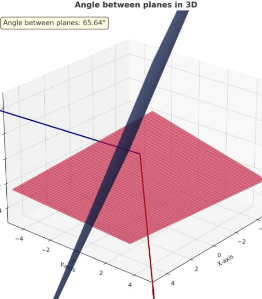
\includegraphics[width=0.8\textwidth]{fig2.2.29}
    \caption{}
    \label{fig:1.2.27.jpg}
\end{figure}

\end{document}